% 问题三·子问题一：M0 的 N-D 基线优化
% 本文件为正文片段，遵循 paper/main.tex 的唯一入口约定；不定义文档环境。
% 证据运行：q3-nd-baseline-20260925-r01。

\subsection{问题三子问题一：M0 的 $N$--$D$ 基线优化}
\label{sec:q3-m0-nd}

问题三子问题一研究给定算力预算和上下文长度下参数规模 $N$ 与训练数据规模
$D$ 的资源分配。为保持问题二中不同数据角色的边界，本节固定
$Q=Q_0$、$p=p_0$，采用 B1/Pythia 条件下的 $N$--$D$ 标度律，
不能直接解释为跨来源的联合最优配置。

本节使用问题二 M0 的 B1/Pythia 拟合参数
\[
E=1.689798,\qquad
A=0.353980,\qquad
B=1.240306,\qquad
\alpha=0.339977,\qquad
\beta=0.279878 .
\]
其中 $N$ 以十亿参数（B）计，$D$ 以十亿 token（B）计。B1 的观测支持域为
\[
N\in[0.070542,11.965825],\qquad
D\in[0.134,299.893].
\]

\subsubsection{解析解}
\label{sec:q3-m0-nd-analytic}

在 $Q$ 和 $p$ 固定时，M0 的预测损失函数为
\begin{equation}
\widehat L(N,D)=E+A N^{-\alpha}+B D^{-\beta}.
\label{eq:q3-m0-loss}
\end{equation}

上下文长度 $L_{\rm ctx}$ 由 C7 架构元数据外生给定，考虑长文本注意力开销后，预算约束按十亿单位换算为
\begin{equation}
10^{18}\bigl(6+\eta L_{\rm ctx}\bigr)ND\le C,
\qquad \eta=2\times10^{-4}.
\label{eq:q3-m0-budget}
\end{equation}
记预算允许的规模乘积为
\begin{equation}
K(C,L_{\rm ctx})
=\frac{C}{10^{18}\bigl(6+\eta L_{\rm ctx}\bigr)}.
\label{eq:q3-m0-k}
\end{equation}

由于 $A,B,\alpha,\beta>0$，有
\begin{equation}
\frac{\partial \widehat L}{\partial N}
=-\alpha A N^{-\alpha-1}<0,\qquad
\frac{\partial \widehat L}{\partial D}
=-\beta B D^{-\beta-1}<0.
\label{eq:q3-m0-first-derivative}
\end{equation}
在不考虑支持域上界时，最优点会用尽预算，即 $ND=K$。将等式约束代入
拉格朗日一阶条件，得到
\begin{equation}
\alpha A N^{-\alpha}=\beta B D^{-\beta},
\qquad ND=K .
\label{eq:q3-m0-balance}
\end{equation}
由此得到预算约束下的无界解析解
\begin{equation}
N_{\rm rel}^{*}
=\left(\frac{\alpha A}{\beta B}K^{\beta}\right)^{1/(\alpha+\beta)},
\qquad
D_{\rm rel}^{*}=\frac{K}{N_{\rm rel}^{*}} .
\label{eq:q3-m0-analytic-solution}
\end{equation}

式~\eqref{eq:q3-m0-balance} 表明，最优分配并不是令 $N$ 和 $D$ 的原始
边际收益相等，而是令两项的弹性加权贡献相等。边际收益递减可由二阶导数
直接验证：
\begin{equation}
\frac{\partial^2\widehat L}{\partial N^2}
=\alpha(\alpha+1)A N^{-\alpha-2}>0,\qquad
\frac{\partial^2\widehat L}{\partial D^2}
=\beta(\beta+1)B D^{-\beta-2}>0 .
\label{eq:q3-m0-diminishing-return}
\end{equation}
因此，增加 $N$ 或 $D$ 均能降低 Loss，但单位资源带来的下降幅度会随相应
资源规模增大而减小。解析解只有在
$(N_{\rm rel}^{*},D_{\rm rel}^{*})$ 落在 B1 支持域内时，才可被解释为
支持域内候选。

C7 中观测到的上下文长度为
\[
L_{\rm ctx}\in\{2048,4096,8192,32768,131072\}.
\]
注意力项系数与基础训练项系数相等的临界上下文长度为
\begin{equation}
L_{\rm ctx}^{\rm crit}=\frac{6}{\eta}=30000.
\label{eq:q3-m0-critical-context}
\end{equation}
该临界值位于 $8192$ 和 $32768$ 之间，因此这两个相邻的 C7 取值可以
用于观察注意力开销跨过临界水平时的资源收缩现象。

\subsubsection{有界数值求解}
\label{sec:q3-m0-nd-bounded}

解析解没有考虑 B1 的观测支持边界。为避免把超出观测范围的点误写成已验证
配置，进一步求解
\begin{equation}
\begin{aligned}
\min_{N,D}\quad &\widehat L(N,D)\\
\mathrm{s.t.}\quad
&ND\le K(C,L_{\rm ctx}),\\
&0.070542\le N\le11.965825,\\
&0.134\le D\le299.893 .
\end{aligned}
\label{eq:q3-m0-bounded-problem}
\end{equation}

数值求解在 $(\log N,\log D)$ 空间中进行，以保持正值并改善不同量级下的
数值条件。每个预算--上下文情景使用六个确定性起点：无界解析解、四个
支持域角点和对数尺度中心点；随后采用带显式预算不等式的 SLSQP 求解。
候选解只有在预算残差满足
\begin{equation}
C-10^{18}\bigl(6+\eta L_{\rm ctx}\bigr)ND
\ge -\max\{1,10^{-10}C\}
\label{eq:q3-m0-feasibility}
\end{equation}
时才保留，并在保留的可行解中选择预测 Loss 最小者。该过程同时检查
预算可行性、$N,D$ 边界可行性和多起点结果的一致性。

15 个场景均得到有限的可行解。每个场景均保留六个起点，成功标记数为
5 或 6，个别场景出现两个数值上不同的情况，按预测 Loss 值选出的
结果与解析解在支持域内部一致到表中展示精度。

\subsubsection{结果分析}
\label{sec:q3-m0-nd-results}

表~\ref{tab:q3-m0-nd-scenarios} 汇总 15 个预算--上下文情景。
$N_{\rm rel}^{*},D_{\rm rel}^{*}$ 表示不加支持域边界的解析解，$N^{*},D^{*}$
表示有界 SLSQP 解。“$D_{\max}$”和“$N_{\max},D_{\max}$”表示有界解
触及相应 B1 支持上界；“域内”和“外推”针对无界解析解判定。

\begin{table}[htbp]
  \centering
  \caption{M0 在 15 个预算--上下文情景下的解析解与有界解}
  \label{tab:q3-m0-nd-scenarios}
  \scriptsize
  \setlength{\tabcolsep}{3pt}
  \renewcommand{\arraystretch}{1.12}
  \resizebox{\textwidth}{!}{%
  \begin{tabular}{rrrrrrrrll}
    \toprule
    $C$ (FLOPs) & $L_{\rm ctx}$ & $N_{\rm rel}^{*}$ & $D_{\rm rel}^{*}$
      & 解析 Loss & $N^{*}$ & $D^{*}$ & 有界 Loss
      & 边界 &求解范围\\
    \midrule
    $10^{19}$ & 2,048   & 0.2213 & 7.0497    & 2.9989 & 0.2213 & 7.0497   & 2.9989 & -- & 域内\\
    $10^{19}$ & 4,096   & 0.2152 & 6.8142    & 3.0114 & 0.2152 & 6.8142   & 3.0114 & -- & 域内\\
    $10^{19}$ & 8,192   & 0.2045 & 6.4031    & 3.0347 & 0.2045 & 6.4031   & 3.0347 & -- & 域内\\
    $10^{19}$ & 32,768  & 0.1634 & 4.8758    & 3.1412 & 0.1634 & 4.8758   & 3.1412 & -- & 域内\\
    $10^{19}$ & 131,072 & 0.1068 & 2.9078    & 3.3672 & 0.1068 & 2.9078   & 3.3672 & -- & 域内\\
    \midrule
    $10^{22}$ & 2,048   & 5.0069  & 311.6048  & 2.1432 & 5.2024 & 299.8930 & 2.1432 & $D_{\max}$ & 外推\\
    $10^{22}$ & 4,096   & 4.8688  & 301.1956  & 2.1475 & 4.8899 & 299.8930 & 2.1475 & $D_{\max}$ & 外推\\
    $10^{22}$ & 8,192   & 4.6256  & 283.0256  & 2.1556 & 4.6256 & 283.0256 & 2.1556 & -- & 域内\\
    $10^{22}$ & 32,768  & 3.6961  & 215.5177  & 2.1925 & 3.6961 & 215.5177 & 2.1925 & -- & 域内\\
    $10^{22}$ & 131,072 & 2.4152  & 128.5289  & 2.2707 & 2.4152 & 128.5290 & 2.2707 & -- & 域内\\
    \midrule
    $10^{24}$ & 2,048   & 40.0506 & 3,895.4695 & 1.9134 & 11.9658 & 299.8930 & 2.0934 & $N_{\max},D_{\max}$ & 外推\\
    $10^{24}$ & 4,096   & 38.9459 & 3,765.3416 & 1.9155 & 11.9658 & 299.8930 & 2.0934 & $N_{\max},D_{\max}$ & 外推\\
    $10^{24}$ & 8,192   & 37.0012 & 3,538.1924 & 1.9195 & 11.9658 & 299.8930 & 2.0934 & $N_{\max},D_{\max}$ & 外推\\
    $10^{24}$ & 32,768  & 29.5660 & 2,694.2546 & 1.9377 & 11.9658 & 299.8930 & 2.0934 & $N_{\max},D_{\max}$ & 外推\\
    $10^{24}$ & 131,072 & 19.3194 & 1,606.7809 & 1.9763 & 11.9658 & 299.8930 & 2.0934 & $N_{\max},D_{\max}$ & 外推\\
    \bottomrule
  \end{tabular}}
\end{table}

低预算 $10^{19}$ FLOPs 下，5 个上下文情景的解析解全部位于 B1 支持域内，
因此解析解与有界解重合。随着上下文从 2,048 增加到 131,072，$N^{*}$
从 0.2213 B 降至 0.1068 B，$D^{*}$ 从 7.0497 B tokens 降至 2.9078 B
tokens，Loss 从 2.9989 上升至 3.3672。这一变化来源于有效规模乘积 $K$
的减少。

中预算 $10^{22}$ FLOPs 下，$L_{\rm ctx}=2,048$ 和 $4,096$ 的无界解析解
分别给出 $D=311.6048$ B 和 $D=301.1956$ B，超过 B1 的
$D_{\max}=299.893$ B；有界求解把 $D$ 截在上界，并相应调整 $N$。
当上下文为 $8,192$ 或更大时，解析解重新回到 B1 支持域内部。因此，
该预算档同时展示了“支持域边界触及”和“上下文开销收缩后回到域内”两种情况。

高预算 $10^{24}$ FLOPs 下，5 个上下文情景的无界解析解都超出 B1 支持域，
且同时超过 $N_{\max}$ 与 $D_{\max}$。有界解在全部情景中均取
$N^{*}=11.965825$ B、$D^{*}=299.893$ B tokens，预测 Loss 均为 2.0934。
由于支持域上界已经限制了可用规模，实际消耗的算力仅约为
$2.30\times10^{22}$ 至 $1.16\times10^{23}$ FLOPs；未使用的预算不能
被解释为模型还可以在 B1 证据范围内继续获得的收益。高预算下无界解析
Loss（1.9134--1.9763）只能作为外推诊断，不能作为已验证的最优 Loss。


图~\ref{fig:q3-m0-nd-baseline}将表中的解析解、有界解和 B1 支持边界放在同一
$N$--$D$ 平面中。低预算点位于观测支持域内部，解析点与有界点基本重合；预算
升高后，解析前沿继续向支持域外延伸，而有界解在 $N_{\max}$ 或 $D_{\max}$
处停止。因而图中的边界点表达的是“在当前支持域内可取的最大配置”，不是对
支持域外模型规模的经验验证。

\begin{figure}[htbp]
  \centering
  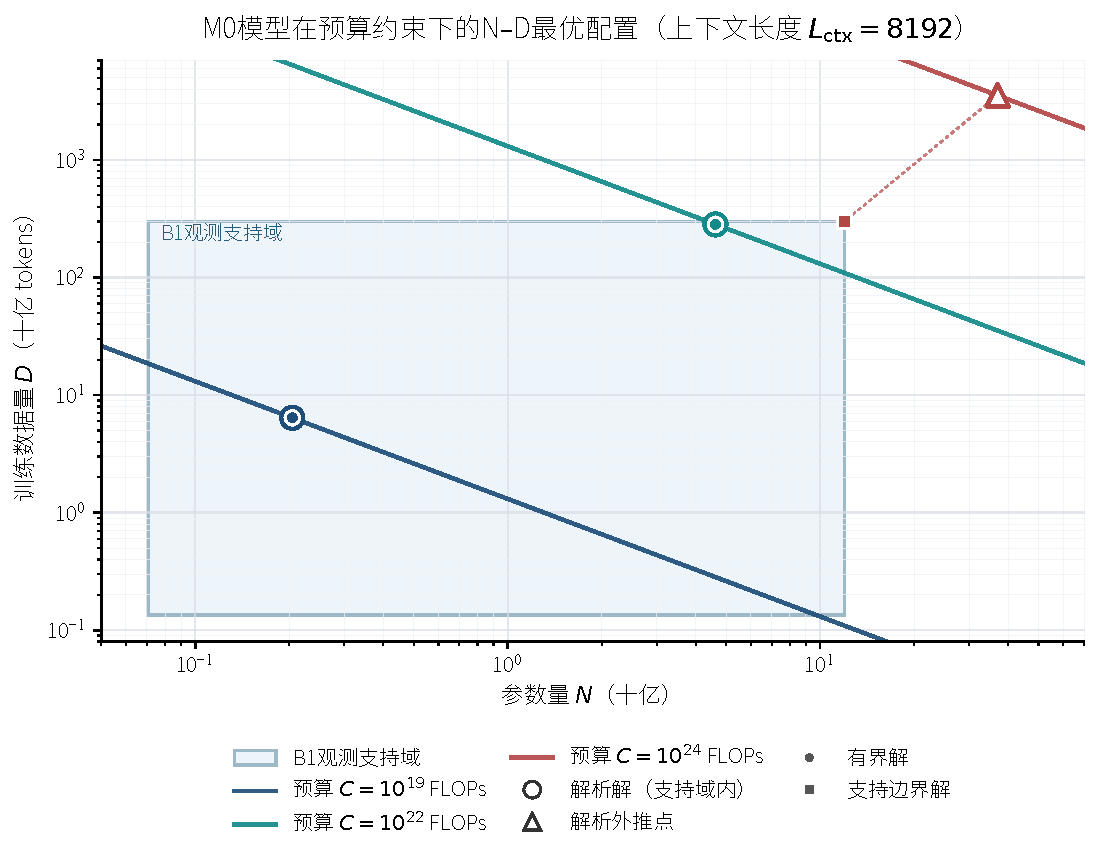
\includegraphics[width=0.82\textwidth]{figures/q3-nd-baseline-cn-v1/fig_q3_m0_nd_cn_single_v1.pdf}
  \caption{M0 在 $L_{\rm ctx}=8192$ 下的 $N$--$D$ 条件配置。空心点表示无界解析解，实心点表示 B1 支持域内的有界解，方形表示支持上界活跃的情景。}
  \label{fig:q3-m0-nd-baseline}
\end{figure}

图~\ref{fig:q3-m0-nd-budget}进一步将五档上下文和三档预算放在同一条件面板中。
随着 $L_{\rm ctx}$ 增加，注意力项压缩有效预算乘积，配置点沿着较低的 $N$--$D$
乘积移动；在 $10^{24}$ FLOPs 档，五个上下文均触及 B1 的双上界。这个图形只
是 15 个场景的可视化索引，数值判定仍以表~\ref{tab:q3-m0-nd-scenarios} 和
支持域约束为准。

\begin{figure}[htbp]
  \centering
  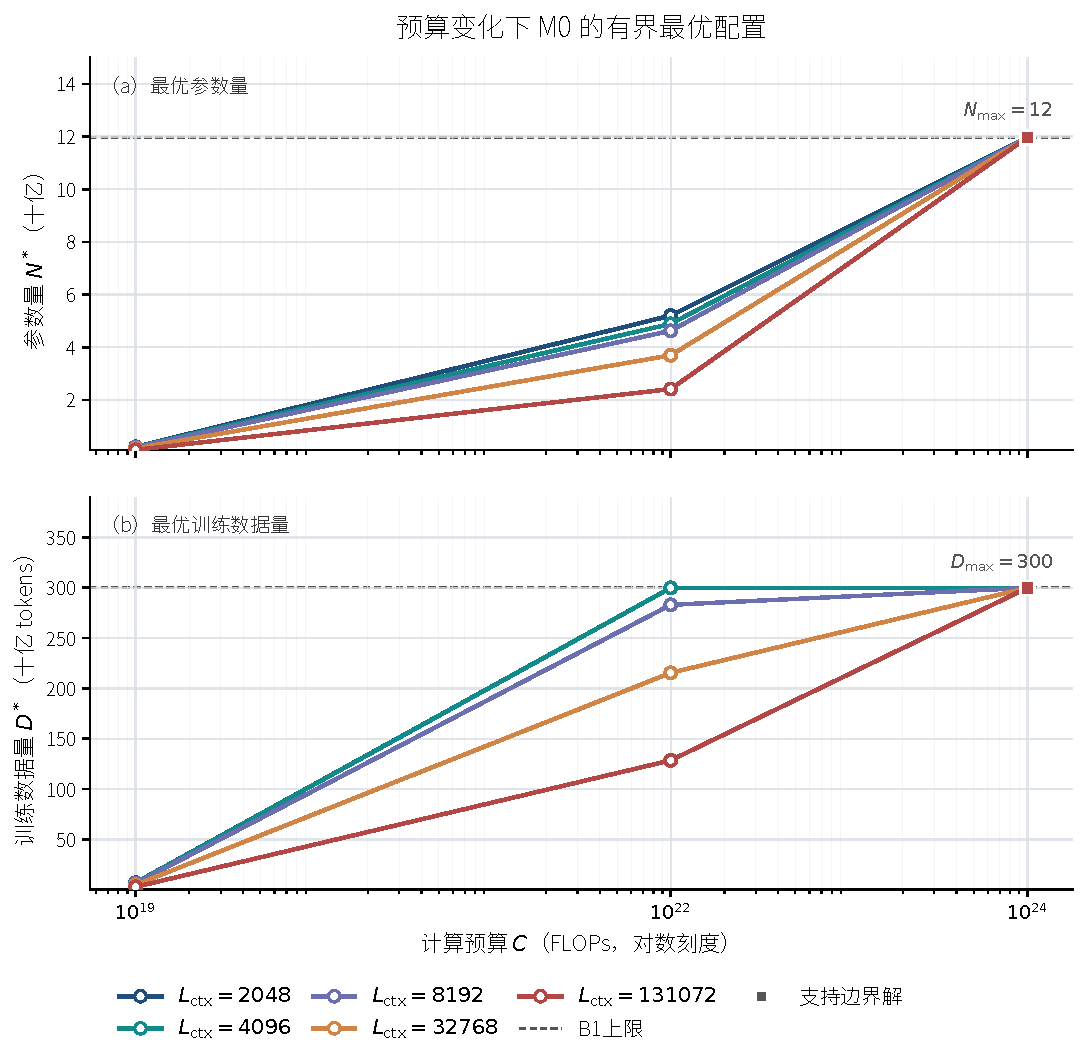
\includegraphics[width=0.78\textwidth]{figures/q3-nd-budget-cn-v1/fig_q3_m0_nd_budget_cn_single_v1.pdf}
  \caption{M0 在三档预算和五档上下文下的有界 $N$--$D$ 配置。虚线表示 B1 观测支持上限，方形表示边界约束活跃的场景。}
  \label{fig:q3-m0-nd-budget}
\end{figure}

\subsubsection{小结}

在 B1/Pythia 的观测支持域内，M0 给出了可复核的 $N$--$D$ 条件资源分配关系。
上下文长度通过注意力成本改变有效预算乘积，支持域上界则决定高预算情景是否
进入边界解。因而本小问的结论是 B1 条件下的规模基线，不能解释为跨来源联合
最优，也不能据此识别质量 $Q$ 或配比 $p$ 的独立作用。参数、支持域、上下文
集合和 15 个情景均来自运行
\begin{center}
{\scriptsize\texttt{q3-nd-baseline-20260925-r01}}
\end{center}
完整结果表为
\texttt{q3\_nd\_baseline\_scenarios.csv}。
